\documentclass[tikz,border=12pt]{standalone}
\usepackage[T1]{fontenc}
\usepackage{mathpazo}
\usepackage{amsmath,amssymb}
\usetikzlibrary{arrows.meta, positioning, calc, fit, decorations.pathreplacing}

\definecolor{stblue}{HTML}{7B97AD}
\definecolor{rwgold}{HTML}{B8995E}
\definecolor{sage}{HTML}{7A9A7E}
\definecolor{dkbrown}{HTML}{3D3530}
\definecolor{wmgray}{HTML}{7B7067}
\definecolor{cream}{HTML}{F9F6F0}
\definecolor{border}{HTML}{D4C9B8}
\definecolor{terracotta}{HTML}{C47A6A}
\definecolor{lavender}{HTML}{907EA0}

\begin{document}
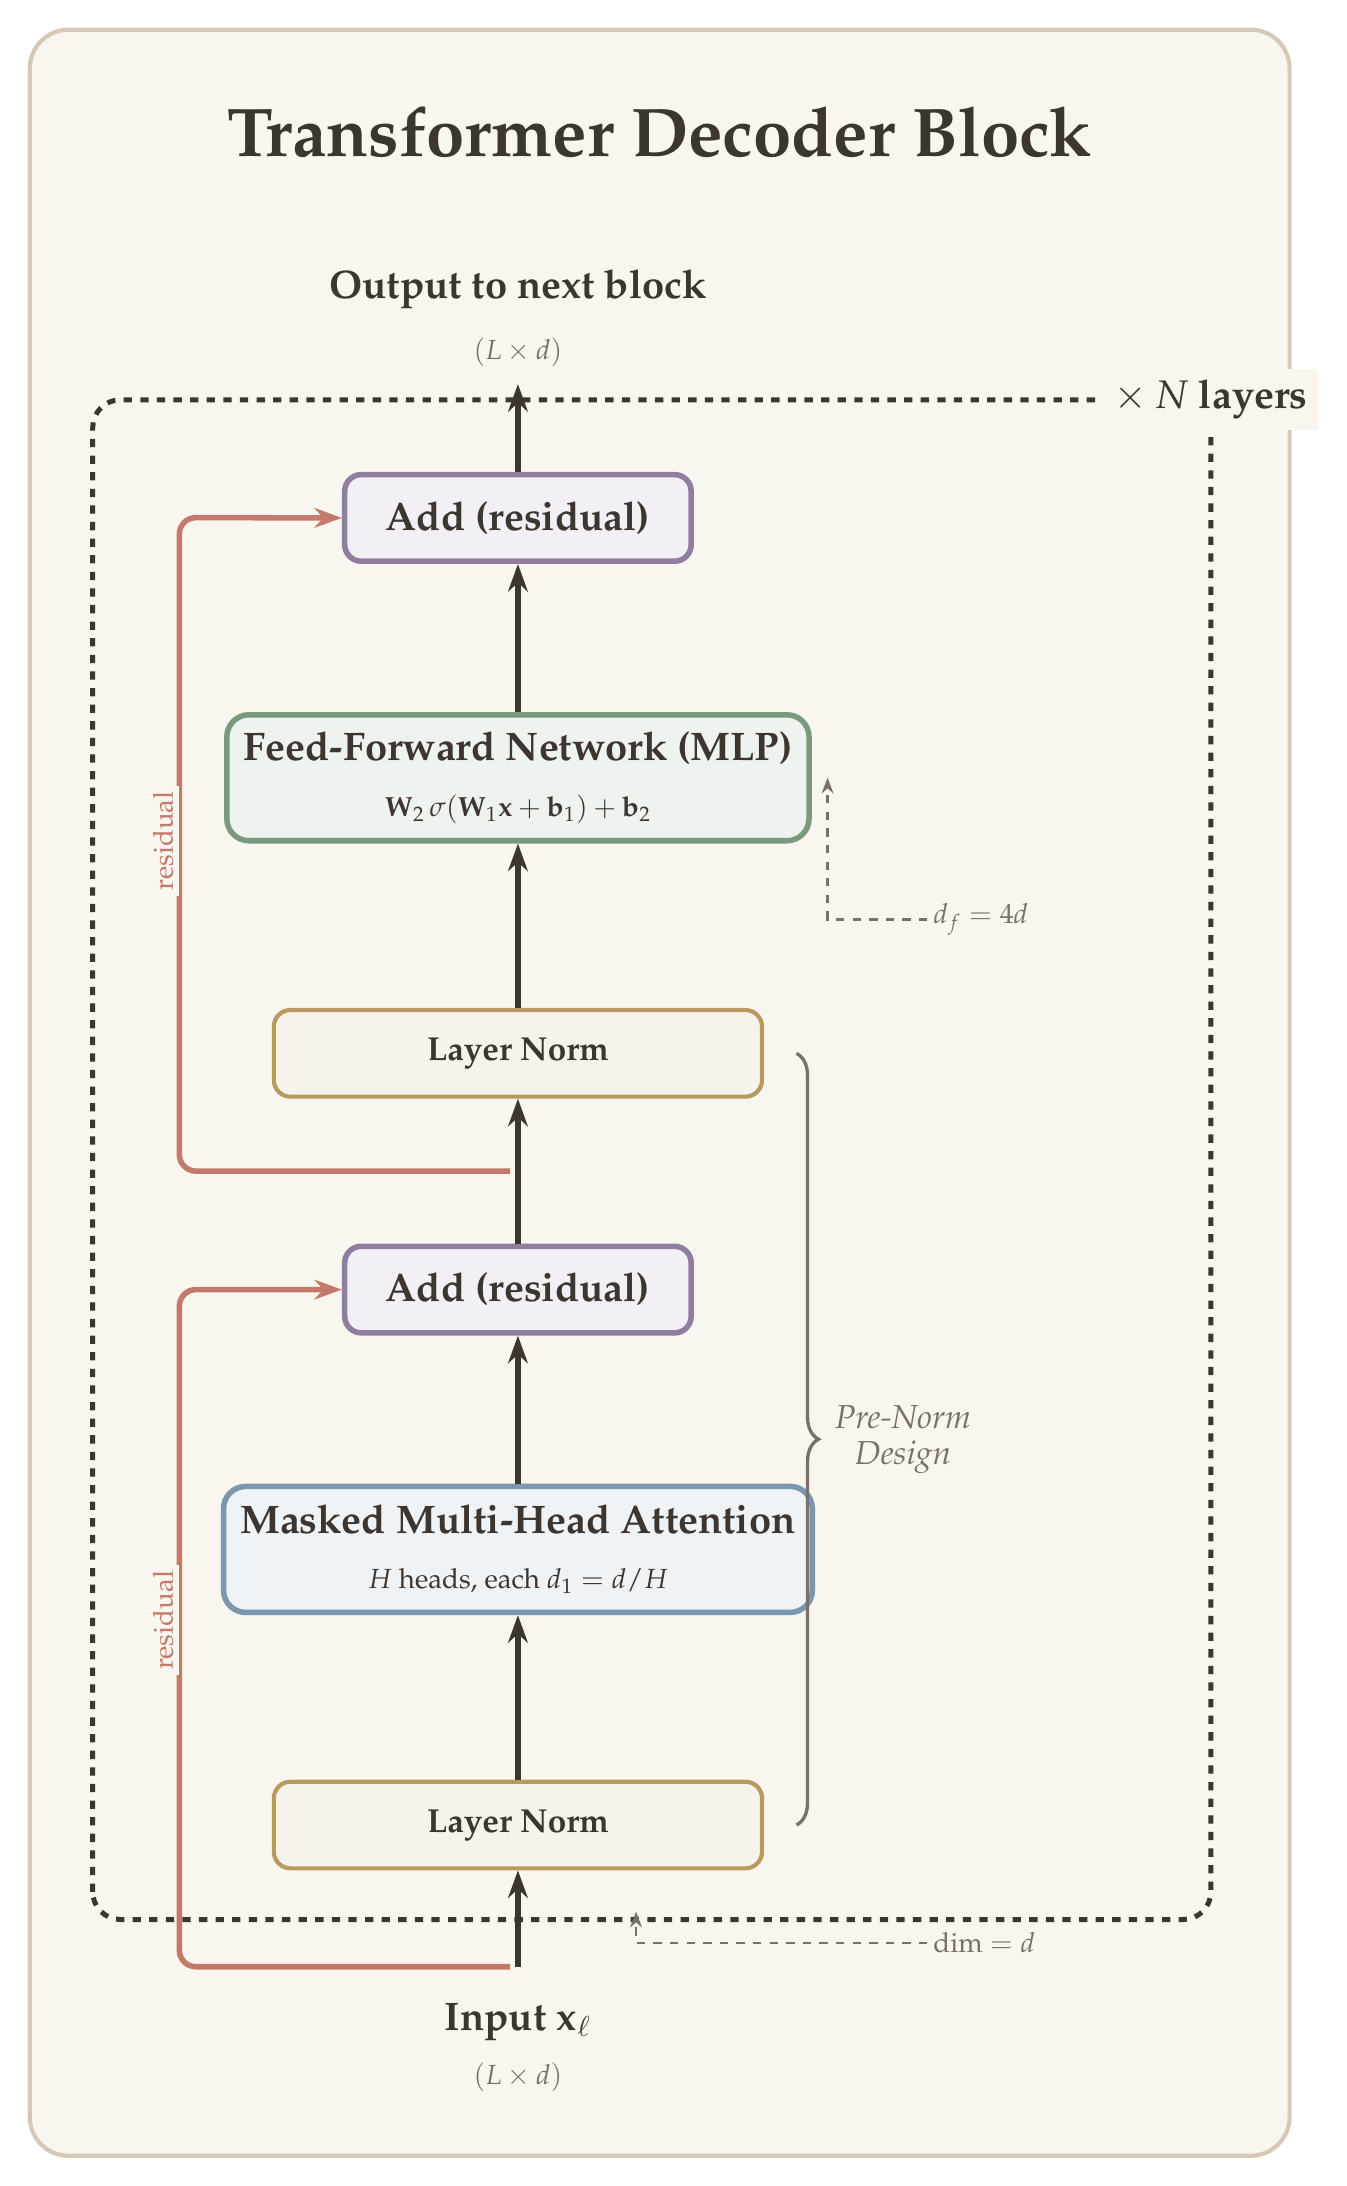
\begin{tikzpicture}[
  >={Stealth[length=3.5mm, width=2.5mm]},
  mainbox/.style={
    draw=#1, line width=2pt, fill=#1!12, rounded corners=8pt,
    minimum width=62mm, minimum height=16mm, font=\Large, text=dkbrown,
    align=center, inner sep=6pt
  },
  normbox/.style={
    draw=rwgold, line width=1.5pt, fill=rwgold!12, rounded corners=6pt,
    minimum width=62mm, minimum height=11mm, font=\large, text=dkbrown,
    align=center, inner sep=5pt
  },
  addnode/.style={
    draw=lavender, line width=2pt, fill=lavender!12, rounded corners=6pt,
    minimum width=44mm, minimum height=11mm, font=\Large\bfseries, text=dkbrown,
    align=center, inner sep=4pt
  },
  arr/.style={->, line width=2pt, dkbrown},
  skiparr/.style={->, line width=2pt, terracotta, rounded corners=6pt},
  annotlabel/.style={font=\normalsize, text=wmgray, fill=cream, inner sep=2pt},
]

% ============================================================
% Background
% ============================================================
\fill[cream, rounded corners=14pt] (-6.2,-4.2) rectangle (9.8,22.8);
\draw[border, rounded corners=14pt, line width=1.5pt] (-6.2,-4.2) rectangle (9.8,22.8);

% Title
\node[font=\Huge\bfseries, text=dkbrown] at (1.8,21.5)
  {Transformer Decoder Block};

% ============================================================
% Main flow: bottom to top (centered at x = 0)
% ============================================================

% --- Input ---
\node[font=\Large\bfseries, text=dkbrown] (input-label) at (0,-2.5)
  {Input $\mathbf{x}_\ell$};
\node[font=\normalsize, text=wmgray] at (0,-3.2) {$(L \times d)$};

% --- Layer Norm 1 ---
\node[normbox] (ln1) at (0,0)
  {\textbf{Layer Norm}};

% --- Masked Multi-Head Attention ---
\node[mainbox=stblue] (mha) at (0,3.5)
  {\textbf{Masked Multi-Head Attention}\\[2pt]
   {\normalsize $H$ heads, each $d_1 = d/H$}};

% --- Add 1 (residual) ---
\node[addnode] (add1) at (0,6.8)
  {Add (residual)};

% --- Layer Norm 2 ---
\node[normbox] (ln2) at (0,9.8)
  {\textbf{Layer Norm}};

% --- Feed-Forward Network ---
\node[mainbox=sage] (ffn) at (0,13.3)
  {\textbf{Feed-Forward Network (MLP)}\\[2pt]
   {\normalsize $\mathbf{W}_2 \,\sigma(\mathbf{W}_1 \mathbf{x} + \mathbf{b}_1) + \mathbf{b}_2$}};

% --- Add 2 (residual) ---
\node[addnode] (add2) at (0,16.6)
  {Add (residual)};

% --- Output ---
\node[font=\normalsize, text=wmgray] (outdim) at (0,18.7) {$(L \times d)$};
\node[font=\Large\bfseries, text=dkbrown] (output-label) at (0,19.5)
  {Output to next block};

% ============================================================
% Main vertical arrows (bottom to top)
% ============================================================
\draw[arr] (0,-1.8) -- (ln1.south);
\draw[arr] (ln1.north) -- (mha.south);
\draw[arr] (mha.north) -- (add1.south);
\draw[arr] (add1.north) -- (ln2.south);
\draw[arr] (ln2.north) -- (ffn.south);
\draw[arr] (ffn.north) -- (add2.south);
\draw[arr] (add2.north) -- (0,18.3);

% ============================================================
% Residual connection 1: bypass LN1 + MHA, into Add1
% ============================================================
\coordinate (res1-start) at (0,-1.8);
\draw[skiparr]
  ([xshift=-1mm]res1-start) -- ++(-4.2,0) -- ++(0,8.6) -- (add1.west);

\node[font=\normalsize, text=terracotta, fill=cream, inner sep=2pt,
      rotate=90, anchor=south]
  at (-4.3,2.6) {residual};

% ============================================================
% Residual connection 2: bypass LN2 + FFN, into Add2
% ============================================================
\coordinate (res2-mid) at ($0.5*(add1.north)+0.5*(ln2.south)$);
\draw[skiparr]
  ([xshift=-1mm]res2-mid) -- ++(-4.2,0) -- ++(0,8.3) -- (add2.west);

\node[font=\normalsize, text=terracotta, fill=cream, inner sep=2pt,
      rotate=90, anchor=south]
  at (-4.3,12.5) {residual};

% ============================================================
% Dashed box: "x N layers"
% ============================================================
\draw[dkbrown, line width=1.8pt, dashed, rounded corners=10pt]
  (-5.4,-1.2) rectangle (8.8,18.1);
\node[font=\Large\bfseries, text=dkbrown, fill=cream, inner sep=4pt]
  at (8.8,18.1) {$\times\, N$ layers};

% ============================================================
% RIGHT-SIDE ANNOTATIONS (inside the dashed box)
% ============================================================

% --- Pre-Norm Design: curly brace connecting both Layer Norms ---
\draw[decorate, decoration={brace, amplitude=8pt, mirror, raise=6pt},
      wmgray, line width=1.2pt]
  ([xshift=2mm]ln1.east) -- ([xshift=2mm]ln2.east)
  node[midway, right=16pt, font=\large\itshape, text=wmgray, align=center]
  {Pre-Norm\\[-1pt]Design};

% --- Dimension annotation: d (horizontal arrow pointing to input wire) ---
\node[annotlabel, anchor=west] (dim-d) at (5.2,-1.5)
  {dim $= d$};
\draw[wmgray, line width=0.8pt, dashed, -{Stealth[length=2mm, width=1.5mm]}]
  (dim-d.west) -- (1.5,-1.5) -- (1.5,-1.1);

% --- Dimension annotation: d_f for FFN hidden (horizontal arrow to FFN) ---
\node[annotlabel, anchor=west] (dim-df) at (5.2,11.5)
  {$d_f = 4d$};
\draw[wmgray, line width=0.8pt, dashed, -{Stealth[length=2mm, width=1.5mm]}]
  (dim-df.west) -- ([xshift=2mm]ffn.east |- 0,11.5) -- ([xshift=2mm]ffn.east);

\end{tikzpicture}
\end{document}
